\documentclass[a4paper]{IEEEtran}
\usepackage{amsmath}
\usepackage{tikz}
\usetikzlibrary{shapes.geometric,arrows,fit,matrix,positioning,shadows}
\usepackage[framemethod=default]{mdframed}
\usepackage{algorithm}
\usepackage{listings}
\usepackage{clrscode}
\usepackage{graphics}
\usepackage{mfirstuc}
\newcommand\addvmargin[1]{
	\node[fit=(current bounding box),inner ysep=#1,inner xsep=0]{};
}
\usepackage[normalem]{ulem}

%\usetikzlibrary{graphs,graphdrawing,arrows.meta,external}

\tikzset
{
    treenode/.style = {circle, draw=black, align=center, minimum size=1cm},
    splitnode/.style = {circle, draw=black, align=center, minimum size=1cm, fill=black!30!white},
    subtree/.style  = {isosceles triangle, draw=black, align=center, minimum height=0.5cm, minimum width=1cm, shape border rotate=90, anchor=north}
    missing/ 
}

\renewcommand\IEEEkeywordsname{Kata Kunci}
\usepackage[bahasa]{babel}
\addto{\captionsbahasa}{\renewcommand{\abstractname}{Abstrak}}
\addto{\captionsbahasa}{\renewcommand*{\refname}{DAFTAR PUSTAKA}
}
\usepackage[utf8]{inputenc}
\usepackage{caption,subcaption}
\usepackage{graphicx}
\usepackage{hyperref}
\usepackage{xesearch}

\usepackage{lettrine}

% Table caption above table
\usepackage{float}
\floatstyle{plaintop}
\restylefloat{table}

% Centering table caption
\usepackage[justification=justified]{caption}

% Prevent hyphenation
\usepackage[none]{hyphenat}


\setcounter{table}{0}
\renewcommand{\thetable}{\arabic{table}}
\renewcommand{\thefigure}{\arabic{figure}}

\usepackage{caption}
\captionsetup[table]{labelsep=period, font=footnotesize}
\captionsetup[figure]{name=Gambar. , labelsep=period, font=footnotesize}
\captionsetup[lstlisting]{labelsep=space, font=footnotesize}

\markboth{\normalsize JURNAL TEKNIK ITS Vol. 4, No. 1, (2015) ISSN: 2337-3539 (2301-9271 Print)}{}
\begin{document}
\title{Penerapan Konsep DSU on Tree dan Struktur Data Segment Tree Pada Rancang Algoritma: Studi Kasus SPOJ Klasik LIS and Tree}
\author{\IEEEauthorblockN{Dimas Hirda Pratama, Rully Soelaiman dan Abdul Munif}\\
\IEEEauthorblockA{Departemen Informatika, Fakultas Teknologi Informasi dan Komunikasi, Institut Teknologi Sepuluh Nopember (ITS)\\
Jl. Arief Rahman Hakim, Surabaya 60111 Indonesia\\
e-mail: dimas14@mhs.if.its.ac.id, rully@is.its.ac.id, munif@if.its.ac.id}}
\maketitle

% ABSTRAK
\begin{abstract}
	 Permasalahan LIS and TREE merupakan sebuah permasalahan yang melibatkan sebuah struktur data tree. Dimana pada tree tersebut akan dicari LIS terpanjang dari seluruh simple path yang ada. Untuk menangani berbagai permasalahan pada permasalahan tersebut dibutuhkan struktur data yang mampu mendukung operasi-operasi tersebut dengan efisien.\\
	 Pada Tugas Akhir ini akan dirancang penyelesaian permasalahan LIS and TREE antara lain operasi pencarian nilai LIS pada node dan subtree saat ini, operasi update nilai LIS pada node dan subtree saat ini dan menggabungkan serta memindahkan nilai pada dua subtree yang berbeda. Struktur data klasik yang biasa digunakan dalam penyelesaian permasalahan ini merupakan salah satu jenis stuktur data Tree yaitu Segment Tree dengan menggabungkan konsep Disjoint Set Union.\\
	 Pada Tugas Akhir ini digunakan struktur data Segment Tree dan konsep Disjoint Set Union untuk menyelesaikan operasi-operasi tersebut.
\end{abstract}
\begin{IEEEkeywords}
	\textit{disjoint set union tree}, \textit{segment tree}, \textit{longest increasing subsequence}
\end{IEEEkeywords}

\section{PENDAHULUAN}

\lettrine[findent=0pt]{\textbf{L}}{IS} and TREE\cite{listree} merupakan permasalahan pencarian \textit{Longest Increasing Subsequence} pada sebuah \textit{tree}, dimana seluruh \textit{node} akan terhubung satu sama lainnya, dengan mengasumsikan seluruh \textit{path} yang ada merupakan \textit{simple path}.\\
Diberikan sejumlah kasus uji dimana pada setiap kasus uji yang ada akan diberikan data berupa bilangan bulat yang menyatakan jumlah \textit{node} pada \textit{tree} dan juga diberikan bilangan bulat $a$ dan $b$ untuk menggambarka bahwa \textit{node} $a$ dan $b$ terhubung oleh \textit{edge}.\\
Penelitian ini akan membahas bagaimana mengetahui hubungan antar \textit{node} dengan menggunakan konsep \textit{disjoint set union on tree} dan mencari nilai LIS pada \textit{tree} tersebut menggunakan bantuan \textit{segment tree}. Gambar \ref{fig:ansvis} menunjukkan contoh bentuk \textit{tree} dari masukan pada situs SPOJ. Tujuan dari penelitian ini adalah menyelesaikan permasalahan, menguji kebenaran dan performa dari algoritma\\
\begin{figure}[H]
	\centering
	\begin{tikzpicture}[level/.style={sibling distance = 5cm/#1, level distance = 1.5cm}, scale=0.64,transform shape]
	\node[treenode]{1}
	child{
		node[treenode,fill=green]{8}
		child{
			node[treenode]{6}
		}
		child{
			node[treenode,fill=green]{3}
			child{
				node[treenode]{12}
			}
			child{
				node[treenode]{10}
			}
			child{
				node[treenode]{5}
				child{
					node[treenode]{4}
				}
				child{
					node[treenode,fill=green]{2}
				}
			}	
		}
	}
	child{
		node[treenode,fill=green]{9}
		child{
			node[treenode,fill=green]{11}
		}
		child{
			node[treenode]{7}
		}	
	};
	\end{tikzpicture}
	\caption{\textit{Node} dengan warna hijau menunjukkan LIS dari contoh masukan pada situs penilaian daring SPOJ\label{fig:ansvis}}
\end{figure}

\section{METODE PENYELESAIAN}
\subsection{Disjoint Set Union}
\quad Struktur data \textit{disjoint set} adalah sebuah struktur data yang menyimpan sekumpulan himpunan atau \textit{set}. Dua himpunan bisa disebut \textit{disjoint} jika kedua himpunan tersebut tidak memiliki perpotongan, atau perpotongannya sama dengan $\textit{null}$. Sebagai contoh himpunan $\{1,2\}$ dan $\{3,4\}$ merupakan himpunan yang \textit{disjoint} karena tidak memiliki elemen yang sama diantara keduanya.\\
\textit{Disjoint set union} sendiri merupakan suatu algoritma yang digunakan untuk menyatukan himpunan yang \textit{disjoint} dengan himpunan lainnya. Hal ini dapat dilakukan dengan melakukan operasi \textit{$merge(a,b)$}, dimana $a$ dan $b$ adalah dua himpunan yang saling \textit{disjoint}.\\
\textbf{Contoh}:\\
\quad Dimisalkan terdapat $5$ buah himpunan bagian yang memiliki anggota berjumlah $1$ yaitu: $\{1\}$, $\{2\}$, $\{3\}$, $\{4\}$, dan $\{5\}$. Kemudian dilakukan operasi seperti pada Gambar \ref{figure:visdsu1} dan \ref{figure:visdsu2}.\\
\begin{figure}[H]
	\centerline{ 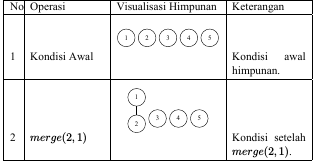
\includegraphics[scale=0.5]{images/tabel1.png}}
	\caption{Visualisasi bentuk \textit{tree} dari contoh masukan}
	\label{figure:visdsu1}
\end{figure}
\begin{figure}
	\centerline{ 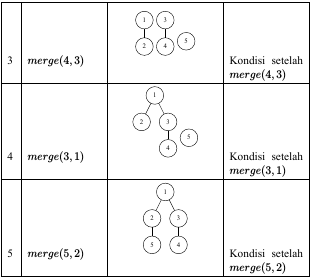
\includegraphics[scale=0.5]{images/tabel2.png}}
	\caption{Visualisasi bentuk \textit{tree} dari contoh masukan}
	\label{figure:visdsu2}
\end{figure}
\subsection{Segment Tree}
\quad\textit{Segment Tree} merupakan salah satu jenis struktur data yang merepresentasikan suatu nilai yang terhubung dengan suatu jeda atau interval tertentu di dalam \textit{array}\cite{ST}. \textit{Segment tree} juga merupakan \textit{binary tree} dimana setiap \textit{node} memiliki maksimal 2 \textit{child}, biasa disebut \textit{left} dan \textit{right} child. Secara umum untuk mengakses nilai didalamnya bisa menggunakan \textit{index} atau \textit{pointer}.
Dimisalkan terdapat sebuah struktur data \textit{segment tree} yang menyimpan interval untuk suatu \textit{array} $A[]$ dengan panjang $n$.Maka rumusan algoritma yang dapat digunakan untuk konstruksi \textit{segment tree} sebagai berikut\cite{ST2}:
\begin{enumerate}
	\item Buat node yang berisikan seluruh elemen \textit{array} $A[]$.
	\item Jika elemen di dalam node beranggotakan lebih dari satu, maka buat $2$ \textit{child node} baru yang beranggotakan elemen $A[0,... .,n/2]$ dan $A[(n/2)+1,... .,n]$.
	\item Jika elemen di dalam node hanya beranggotakan 1 elemen maka proses dihentikan.
\end{enumerate}
\quad Pada Gambar \ref{fig:subbentukST1} menunjukkan  \textit{node} yang menyimpan nilai dari seluruh rentang yang ada menjadi \textit{root} dari \textit{segment tree}.
\begin{figure}[H]
	\begin{subfigure}{.5\textwidth}
		\centering
		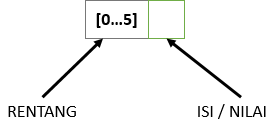
\includegraphics[scale=0.45]{images/pembentukan_ST_1.PNG}
		\caption{}
		\label{fig:subbentukST1}
	\end{subfigure}
	\begin{subfigure}{.5\textwidth}
		\centering
		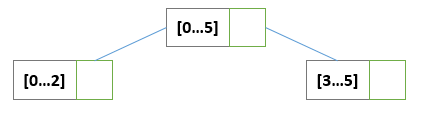
\includegraphics[scale=0.45]{images/pembentukan_ST_2.PNG}
		\caption{}
		\label{fig:subbentukST2}
	\end{subfigure}
	\begin{subfigure}{.5\textwidth}
		\centering 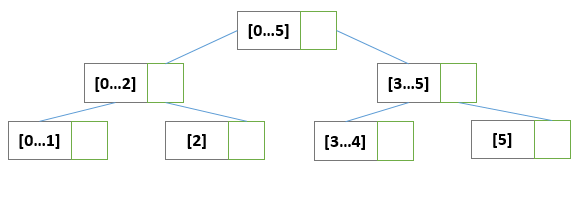
\includegraphics[scale=0.3]{images/pembentukan_ST_3.PNG}
		\caption{}
		\label{fig:subbentukST3}
	\end{subfigure}
	\begin{subfigure}{.5\textwidth}
		\centering
		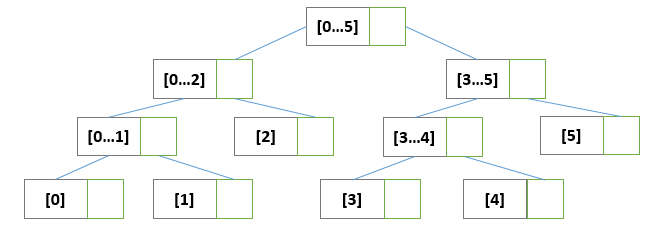
\includegraphics[scale=0.3]{images/pembentukan_ST_4.PNG}
		\caption{}
		\label{fig:subbentukST4}
	\end{subfigure}	
	\caption{Proses pembentukan \textit{Segment Tree}}
	\label{fig:bentukST1}
\end{figure}
Gambar \ref{fig:subbentukST2} menunjukkan proses rekursi untuk membuat dua \textit{child} baru, \textit{child} kiri menyimpan nilai dari rentang 0 hingga 2, \textit{child} kanan menyimpan nilai dari rentang 3 hingga 5. Gambar \ref{fig:subbentukST3} menunjukkan lanjutan proses rekursi lagi, namun untuk \textit{node} yang menyimpan hanya satu rentang saja, yaitu \textit{node} yang menyimpan rentang 2 dan 5 proses dihentikan, bentuk akhir dari \textit{segment tree} terlihat pada Gambar \ref{fig:subbentukST4}.\\
Selain itu pada umumnya struktur data \textit{segment tree} juga memiliki fungsi \textit{$query()$} untuk mengambil nilai dari suatu rentang dan juga \textit{$update()$} untuk merubah nilai pada suatu rentang.\\
Algoritma untuk melakukan fungsi \textit{$query()$} sebagai berikut:
\begin{enumerate}
	\item Cek apakah nilai dari rentang yang diinginkan berada dalam rentang saat ini.
	\item Jika iya ambil nilai yang berada di rentang tersebut.
	\item Jika tidak lakukan rekursi ke \textit{left child} dan \textit{right child}.
\end{enumerate}
Algoritma untuk melakukan fungsi \textit{$update()$} sebagai berikut:
\begin{enumerate}
	\item Cek apakah nilai dari rentang yang diinginkan berada dalam rentang saat ini.
	\item Jika iya ambil \textit{update} nilai yang berada di rentang tersebut.
	\item Jika tidak lakukan rekursi ke \textit{left child} dan \textit{right child}.
\end{enumerate}
\subsection{Heavy-Light Decomposition}
\textit{Heavy-Light Decomposition} adalah teknik dekomposisi sebuah \textit{tree} menjadi sebuah \textit{disjoint chains} (tidak ada 2 \textit{chain} yang memiliki \textit{node} yang sama). Disebut \textit{Heavy-Light} karena dekomposisi dilakukan berdasarkan kriteria yang telah ditentukan untuk membedakan apakah \textit{chain} tersebut merupakan \textit{node heavy} atau \textit{light}.

\quad Penggunaan konsep \textit{Heavy-Light Decomposition}, yakni mengumpamakan sebuah \textit{node} mempunyai satu \textit{special child} yang merupakan sebuah \textit{subtree} dengan ukuran paling besar di antara \textit{child} lainnya. sehingga dapat diumpamakan \textit{tree} yang telah dibuat terdiri dari beberapa \textit{chain} dimana setiap \textit{chain} mempunyai \textit{head} yang bukan merupakan \textit{special child} dari \textit{parent child} tersebut.

\quad Setelah membentuk \textit{tree}, selanjutnya dicatat \textit{edge} mana yang merupakan \textit{heavy edge} dan \textit{light edge}. Dengan aturan berikut:
\begin{enumerate}
\item \textit{Heavy edge} adalah \textit{edge} dengan jumlah \textit{child} lebih besar atau sama dengan setengah jumlah \textit{child} dari \textit{parent child} tersebut.
\item \textit{Light edge} adalah \textit{edge} dengan jumlah \textit{child} kurang dari setengah jumlah \textit{child} dari \textit{parent child} tersebut.
\end{enumerate}
\quad Pada Gambar \ref{fig:ht} dapat dilihat terdapat banyak warna berbeda, setiap warna menggambarkan \textit{chain} yang berbeda, dan \textit{heavy chain} untuk \textit{tree} tersebut ditandai dengan warna hijau.
\begin{figure}[H]
\centering
\begin{tikzpicture}[level/.style={sibling distance = 5cm/#1, level distance = 1.5cm}, scale=0.68,transform shape]
\node[treenode,fill=green]{1}
child{
node[treenode,fill=green]{2}
child{
node[treenode,fill=yellow]{5}
}
child{
node[treenode,fill=green]{6}
child{
node[treenode,fill=green]{8}
child{
node[treenode,fill=green]{10}
}
child{
node[treenode,fill=brown]{11}
}
}
}
}
child{
node[treenode,fill=cyan]{3}
child{
node[treenode,fill=cyan]{7}
child{
	node[treenode,fill=cyan]{9}
	}
	}
	}
	child{
		node[treenode,fill=pink]{4}
		};
		\end{tikzpicture}
		\caption{Contoh penggambaran \textit{Heavy-Light Decomposition}\label{fig:ht}}
		\end{figure}
\subsection{Longest Increasing Subsequence}
Dalam ilmu komputer, permasalahan \textit{Longest Increasing Subsequence} atau yang biasa disingkat menjadi LIS, merupakan permasalahan yang bertujuan untuk menemukan \textit{subsequence} terpanjang dari sebuah \textit{sequence} dimana \textit{subsequence} tersebut memiliki elemen yang sudah disortir dari nilai terkecil ke terbesar.\\
Untuk dapat menyelesaikannya algoritma yang dibutuhkan adalah sebagai berikut:\\
Dimisalkan terdapat sebuah \textit{array} bernama $A[]$ yang memiliki panjang tertentu, dan penulis juga memiliki LIS terpanjang sementara atau disebut \textit{active list} dengan panjang tertentu. Kemudian penulis ingin menambahkan elemen ke-\textit{i} atau $A[\textit{i}]$ maka harus memperhatikan beberapa hal sebagai berikut\cite{LIS}:
\begin{enumerate}
	\item jika $A[\textit{i}]$ adalah elemen terkecil dari \textit{active list} maka buat \textit{active list} baru dengan panjang $1$.
	\item Jika $A[\textit{i}]$ adalah elemen terbesar dari \textit{active list} maka lakukan duplikasi terhadap \textit{active list} terpanjang dan tambahkan elemen tersebut di akhir.
	\item Jika $A[\textit{i}]$ bukan elemen terbesar ataupun terkecil maka cari \textit{active list} dengan elemen terakhir yang terbesar dan lebih kecil dari $A[\textit{i}]$, lakukan duplikasi dan tambahkan elemen tersebut, dan hapus \textit{list} lain dengan panjang yang sama.
\end{enumerate}
\textbf{Contoh}\\
Untuk menemukan LIS dari array $A[0,8,4,12,2,10,14]$
\begin{enumerate}
	\item $A[0]$ = $1$, karena merupakan elemen pertama dan belum ada \textit{active list} maka masuk ke \textit{case} 1.\\\\
	$[0]$\\
	\item $A[1]$ = $8$, karena angka $8$ lebih besar daripada $0$, maka masuk ke \textit{case} 2.\\\\
	$[0]$\\
	$[0,8]$\\
	\item $A[2]$ = $4$, karena angka $4$ berada di antara $0$ dan $8$, maka akan masuk ke \textit{case} 3.\\\\
	$[0]$\\
	$[0,4]$\\
	\sout{$[0,8]$} (dihilangkan)\\
	\item $A[3]$ = $12$, karena angka $12$ lebih besar daripada $4$, maka masuk ke \textit{case} 1.\\\\
	$[0]$\\
	$[0,4]$\\
	$[0,4,12]$\\\\
	\item $A[4]$ = $2$, karena angka $2$ berada di antara $0$ dan $12$ maka akan masuk ke \textit{case} 3.\\\\
	$[0]$\\
	$[0,2]$\\
	\sout{$[0,4]$} (dihilangkan)\\
	$[0,4,12]$\\
	\item $A[5]$ = $10$, karena angka $10$ berada di antara $0$ dan $12$ maka akan masuk ke \textit{case} 3.\\\\
	$[0]$\\
	$[0,2]$\\
	$[0,2,10]$\\
	\sout{$[0,4,12]$} (dihilangkan)\\
	\item $A[6]$ = $14$, karena angka $14$ lebih besar daripada $10$ maka akan masuk ke \textit{case} 1.\\\\
	$[0]$\\
	$[0,2]$\\
	$[0,2,10]$\\
	$[0,2,10,14]$\\ merupakan LIS dari array tersebut.
\end{enumerate}
\subsection{Strategi Penyelesaian}
Dalam persoalan \textit{LIS and TREE} LIS yang dicari merupakan sebuah \textit{path} dari \textit{tree} itu sendiri, dan \textit{path} ini merupakan sebuah \textit{simple path}. Maka untuk mendapatkan nilai LIS tersebut, secara umum terdapat beberapa \textit{case} agar mendapatkan nilai LIS dari setiap \textit{path} yang ada.\\
\textit{Case} yang ada adalah sebagai berikut:
\begin{enumerate}
	\item \textit{Case} yang pertama adalah jika nilai \textit{node} yang lebih besar berada di atas \textit{node} tersebut, seperti pada Gambar \ref{fig:case1}. Menunjukkan bahwa nilai \textit{node} $a$ \textgreater $b$, sehingga arah \textit{path} dari bawah menuju ke atas.
	\item \textit{Case} yang kedua adalah jika nilai \textit{node} yang lebih besar berada di bawah \textit{node} tersebut, seperti pada Gambar \ref{fig:case2}. Menunjukkan bahwa nilai \textit{node} $a$ \textless $b$, sehingga arah \textit{path} dari atas menuju ke bawah.
	\item \textit{Case} yang kedua adalah jika nilai \textit{node} yang lebih besar berada di \textit{depth} yang sama dari \textit{node} tersebut, seperti pada Gambar \ref{fig:case3}. Menunjukkan bahwa nilai \textit{node} $a$ \textgreater $b$, sehingga arah \textit{path} dari bawah menuju ke atas kemudian menuju ke bawah.
\end{enumerate} 
\begin{figure}[H]
	\centering
	\begin{tikzpicture}
	[level/.style={sibling distance = 5cm/#1, level distance = 1.5cm}, scale=0.68,transform shape]
	\node[treenode,fill=green]{a}
	child{
		node[treenode]{}
		child{
			node[treenode]{}
		}
		child{
			node[treenode,fill=green]{b}
		}	
	}
	child{
		node[treenode]{}
		child{
			node[treenode]{}
		}
		child{
			node[treenode]{}
		}
	};
	\end{tikzpicture}\caption{Visualisasi \textit{case} 1.\label{fig:case1}}
\end{figure}
\begin{figure}[H]
	\centering
	\begin{tikzpicture}
	[level/.style={sibling distance = 5cm/#1, level distance = 1.5cm}, scale=0.68,transform shape]
	\node[treenode,fill=green]{a}
	child{
		node[treenode]{}
		child{
			node[treenode,fill=green]{b}
		}
		child{
			node[treenode]{}
		}	
	}
	child{
		node[treenode]{}
		child{
			node[treenode]{}
		}
		child{
			node[treenode]{}
		}
	};
	\end{tikzpicture}\caption{Visualisasi \textit{case} 2.\label{fig:case2}}
\end{figure}
\begin{figure}[H]
	\centering
	\begin{tikzpicture}
	[level/.style={sibling distance = 5cm/#1, level distance = 1.5cm}, scale=0.68,transform shape]
	\node[treenode]{}
	child{
		node[treenode]{}
		child{
			node[treenode,fill=green]{a}
		}
		child{
			node[treenode]{}
		}	
	}
	child{
		node[treenode]{}
		child{
			node[treenode]{}
		}
		child{
			node[treenode,fill=green]{b}
		}
	};
	\end{tikzpicture}\caption{Visualisasi \textit{case} 3.\label{fig:case3}}
\end{figure}
Secara umum algoritma penyelesaian yang dilakukan untuk setiap \textit{node} adalah sebagai berikut:
\begin{enumerate}
	\item Tentukan \textit{child} yang menjadi \textit{big child} atau \textit{small child} menggunakan konsep \textit{Heavy-light Decomposition}.
	\item Lakukan rekursi ke \textit{small child}
	\item Lakukan perulangan untuk mencari LIS dan LDS dari \textit{parent} pada seluruh \textit{child} yang bukan merupakan \textit{bigchild}.
	\item Simpan hasil LIS dan LDS tersebut ke \textit{Segment Tree}.
	\item Cari nilai LIS dan LDS dari \textit{child} ke \textit{parent}.
	\item Simpan hasil LIS dan LDS tersebut ke \textit{Segment Tree}.
	\item Setelah selesai, kembalikan \textit{Segment Tree} ke kondisi semula.
	\item Lakukan rekursi ke \textit{big child}.
	\item Ulangi proses ke 3 hingga 6.
	\item Setelah selesai, biarkan kondisi \textit{Segment Tree} karena akan digunakan kembali.
	\item Lakukan proses hingga semua \textit{node} terlewati.
\end{enumerate}
\section{UJI COBA DAN ANALISIS}

\subsection{Uji coba kebenaran}
Uji coba kebenaran dilakukan dengan mengumpulkan berkas kode sumber hasil implementasi ke situs sistem penilaian daring SPOJ kali. Permasalahan yang diselesaikan adalah LIS and TREE dengan kode LISTREE. Hasil uji kebenaran dan waktu eksekusi program saat pengumpulan kasus uji pada situs SPOJ ditunjukkan pada Gambar \ref{figure:accindex} untuk teknik pengaksesan \textit{segment tree} menggunakan \textit{index} dan Gambar \ref{figure:accpointer} untuk teknik pengaksesan \textit{segment tree} menggunakan \textit{pointer}.
\begin{figure}[H]
	\centering
	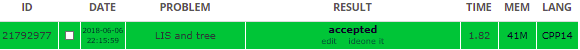
\includegraphics[width=\linewidth]{images/valueacc.png}
	\caption{Hasil uji kebenaran teknik \textit{index} dengan melakukan \textit{submission} ke situs penilaian daring SPOJ}
	\label{figure:accindex}
\end{figure}
\begin{figure}[H]
	\centering
	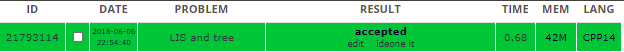
\includegraphics[width=\linewidth]{images/pointeracc.png}
	\caption{Hasil uji kebenaran teknik \textit{pointer} dengan melakukan \textit{submission} ke situs penilaian daring SPOJ}
	\label{figure:accpointer}
\end{figure}
Berikutnya adalah pengujian performa dari algoritma yang dirancang dan diimplementasi dengan melakukan uji \textit{submission} dengan mengumpulkan berkas kode implementasi dari algoritma yang dibangun sebanyak 20 kali ke situs penilaian daring SPOJ dengan mencatat waktu eksekusi serta memori yang dibutuhkan.\\
Hasil dari pengujian untuk teknik pengaksesan \textit{segment tree} menggunakan \textit{index} dapat dilihat pada Gambar \ref{figure:chart} dan Tabel \ref{tab:statistik1}.
\begin{figure}[H]
	\centering
	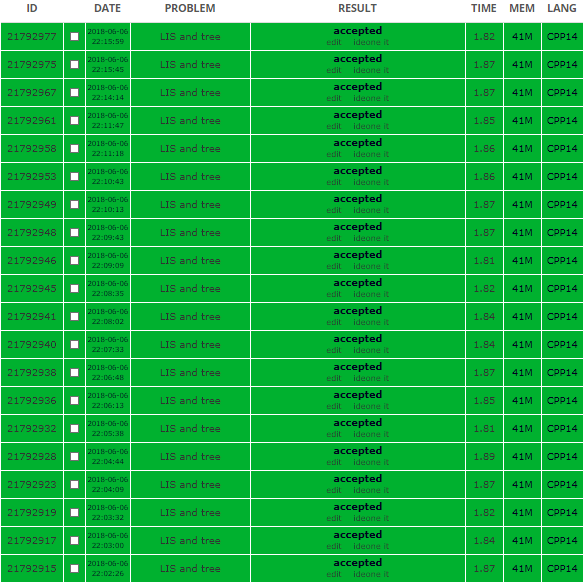
\includegraphics[width=\linewidth]{images/20accST.PNG}
	\caption{Hasil uji coba teknik \textit{index} \textit{submission} ke situs penilaian daring SPOJ sebanyak 20 kali}
	\label{figure:chart}
\end{figure}
\begin{table}[H]
	\centering
	\begin{tabular}{|l|l|} \hline
		Waktu Maksimal & $ 1.89 $ detik\\ \hline
		Waktu Minimal & $ 1.81 $ detik\\ \hline
		Waktu Rata-Rata & $ 1.85 $ detik\\ \hline
		Memori Maksimal & $ 41.0 $ MB\\ \hline
		Memori Minimal & $ 41.0 $ MB\\ \hline
		Memori Rata-Rata & $ 41.0 $ MB\\ \hline
	\end{tabular}
	\caption{Kecepatan maksimal, minimal dan rata-rata dari hasil uji coba pengumpulan teknik \textit{index} sebanyak 20 kali pada situs pengujian daring SPOJ}
	\label{tab:statistik1}
\end{table}
Hasil dari pengujian untuk teknik pengaksesan \textit{segment tree} menggunakan \textit{pointer} dapat dilihat pada Gambar \ref{figure:chart2} dan Tabel \ref{tab:statistik2}.
\begin{figure}[H]
	\centering
	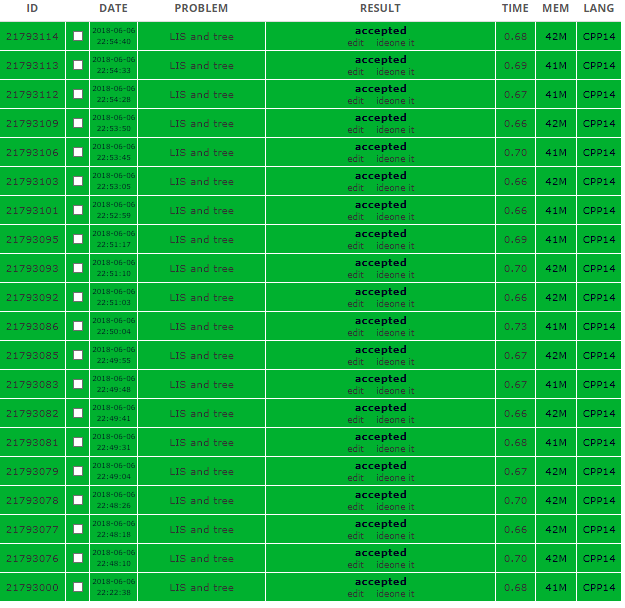
\includegraphics[width=\linewidth]{images/20accP.PNG}
	\caption{Hasil uji coba teknik \textit{pointer} \textit{submission} ke situs penilaian daring SPOJ sebanyak 20 kali}
	\label{figure:chart2}
\end{figure}
\begin{table}[H]
	\centering
	\begin{tabular}{|l|l|} \hline
		Waktu Maksimal & $ 0.73 $ detik\\ \hline
		Waktu Minimal & $ 0.66 $ detik\\ \hline
		Waktu Rata-Rata & $ 0.6795 $ detik\\ \hline
		Memori Maksimal & $ 41.0 $ MB\\ \hline
		Memori Minimal & $ 41.0 $ MB\\ \hline
		Memori Rata-Rata & $ 41.0 $ MB\\ \hline
	\end{tabular}
	\caption{Kecepatan maksimal, minimal dan rata-rata dari hasil uji coba pengumpulan teknik \textit{pointer} sebanyak 20 kali pada situs pengujian daring SPOJ}
	\label{tab:statistik2}
\end{table}
\subsection{Uji Coba Kinerja}
Pada uji coba yang ditunjukkan Gambar \ref{figure:grafnode} terlihat performa program dengan input jumlah kasus uji satu, dan jumlah \textit{node} yang bertambah hingga 100000.
\begin{figure}[H]
	\centerline{ 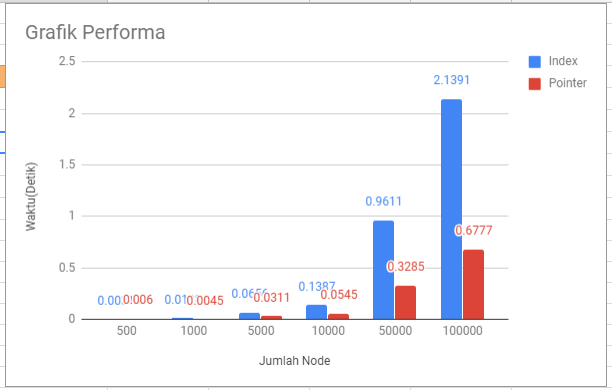
\includegraphics[scale=0.5]{images/GrafikPerformaNode.PNG}}
	\caption{Hasil uji coba program menggunakan data dari generator}
	\label{figure:grafnode}
\end{figure}
Pada gambar grafik berwarna merah menunjukkan performa dari implementasi menggunakan pointer dan warna biru menunjukkan performa dari implementasi menggunakan index. Terlihat perbedaan yang cukup besar ketika masukan mencapai 100000 \textit{node}, hal ini dikarenakan banyaknya bagian \textit{segment tree} yang kosong yang harus dicek pada saat menggunakan implementasi index.
Pada uji coba yang ditunjukkan Gambar \ref{figure:graftestcase} terlihat performa program dengan input jumlah kasus uji yang bertambah hingga 1000, dan jumlah \textit{node} yang konstan yaitu 100000.
\begin{figure}[H]
	\centerline{ 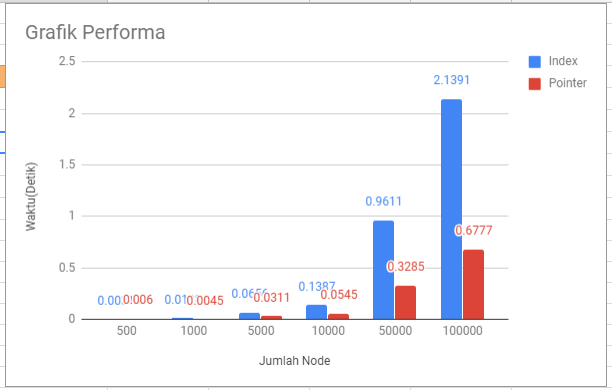
\includegraphics[scale=0.5]{images/GrafikPerformaNode.PNG}}
	\caption{Hasil uji coba program menggunakan data dari generator}
	\label{figure:graftestcase}
\end{figure}
Pada gambar grafik berwarna merah menunjukkan performa dari implementasi menggunakan pointer dan warna biru menunjukkan performa dari implementasi menggunakan index. Waktu disini bertambah seiring dengan banyaknya kasus uji secara konstan.
\subsection{Analisis Kompleksitas}
Kedua teknik penyelesaian baik menggunakan \textit{pointer} atau \textit{index} memiliki kompleksitas yang sama yaitu $O (N \log^2 N)$. Kompleksitas ini didapatkan dari banyaknya proses memindahkan nilai dari \textit{small child} ke \textit{big child} yaitu sebesar $O (N \log N)$ dan proses \textit{$query()$} serta \textit{$update()$} yang dilakukan yaitu sebesar $O (\log N)$ dengan $N$ adalah jumlah dari \textit{node} pada \textit{tree}.
\section{KESIMPULAN}
Dari hasil uji coba yang dilakukan terhadap implementasi penyelesaian permasalahan \textit{LIS and TREE} dapat diambil kesimpulan sebagai berikut:
\begin{enumerate}
	\item Implementasi algoritma \textit{Disjoint Set Union on Tree} dengan struktur data \textit{Segment Tree} dapat menyelesaikan permasalahan \textit{LIS and TREE} dengan benar.
	\item Implementasi algoritma \textit{DSU on TREE} pada struktur data \textit{Segment Tree} dapat menghasilkan kecepatan proses yang berbeda dengan menggunakkan pendekatan yang berbeda yaitu (\textit{by value \text{\&} by reference}).
	\item Kompleksitas waktu yang dibutuhkan untuk seluruh sistem adalah $O(n\log^{2}n)$, dengan $n$ merupakan banyaknya \textit{node} yang ada pada \textit{tree} tersebut.
\end{enumerate}
\section*{UCAPAN TERIMA KASIH}
Penulis mengucapkan puji syukur kehadirat Allah SWT atas segala rahmat dan karunia-Nya sehingga memungkinkan penulis untuk dapat menyelesaikan penelitian ini. Penulis juga mengucapkan terima kasih kepada orang tua dan keluarga penulis, juga kepada Bapak Rully Soelaiman dan Bapak Abdul Munif selaku dosen pembimbing penulis dan kepada semua pihak yang telah memberikan dukungan baik secara langsung maupun tidak langsung selama penulis mengerjakan penelitian ini.

% DAFTAR PUSTAKA
\begin{thebibliography}{9}
	\bibitem{listree}
	Bartek, "LIS and TREE" [Online]. Available: http://www.spoj.com/problems/LISTREE/ . [Accessed 17-May-2018].
	 
	\bibitem{LIS}
	Geeksforgeeks, "Longest Increasing Subsequence" [Online]. Avaiable: http://www.geeksforgeeks.org/longest-monotically-increasing-\\subsequence-size-n-log-n [Accesed 17-May-2018].
	
	\bibitem{ST}
	\textbf{Understanding Segment Trees} - Understanding segment tree · CodingHigway [Online]. Avaiable: http://codinghighway.com/2014/09/13/understanding-segment-\\trees/ [Accessed 17-May-2018].
	
	\bibitem{ST2}
	\textbf{Segment Tree | Set 1 (Sum of given range)} - Segment Tree | Set 1 (Sum of given range) - GeeksforGeeks [Online]. Avaiable: http://www.geeksforgeeks.org/segment-trees-set-1-sum-of-\\given-range/ [Accessed 17-May-2018].
		
\end{thebibliography}
\end{document}
